\documentclass[tikz,border=5pt]{standalone}
\usepackage{fontspec}
\usepackage{amsmath}
\usetikzlibrary{arrows.meta,positioning,fit,backgrounds,calc}
\setmainfont{TeX Gyre Heros}
\definecolor{ink}{HTML}{24364B}
\definecolor{blue}{HTML}{DCEAF7}
\definecolor{teal}{HTML}{DDF1EC}
\definecolor{amber}{HTML}{F7EBCF}
\definecolor{violet}{HTML}{EAE3F4}
\definecolor{muted}{HTML}{66788A}
\tikzset{
  stage/.style={draw=ink,rounded corners=2pt,line width=.75pt,minimum height=34mm,align=center,text=ink},
  flow/.style={-{Latex[length=2.2mm]},line width=1pt,draw=ink},
  family/.style={rounded corners=1.5pt,minimum width=27mm,minimum height=5.8mm,align=left,font=\scriptsize,text=ink},
  tag/.style={rounded corners=4pt,draw=ink!45,fill=white,inner xsep=4pt,inner ysep=2.2pt,font=\scriptsize,text=ink},
  phase/.style={font=\bfseries\scriptsize,text=muted}
}
\begin{document}
\special{pdf:minorversion 5}
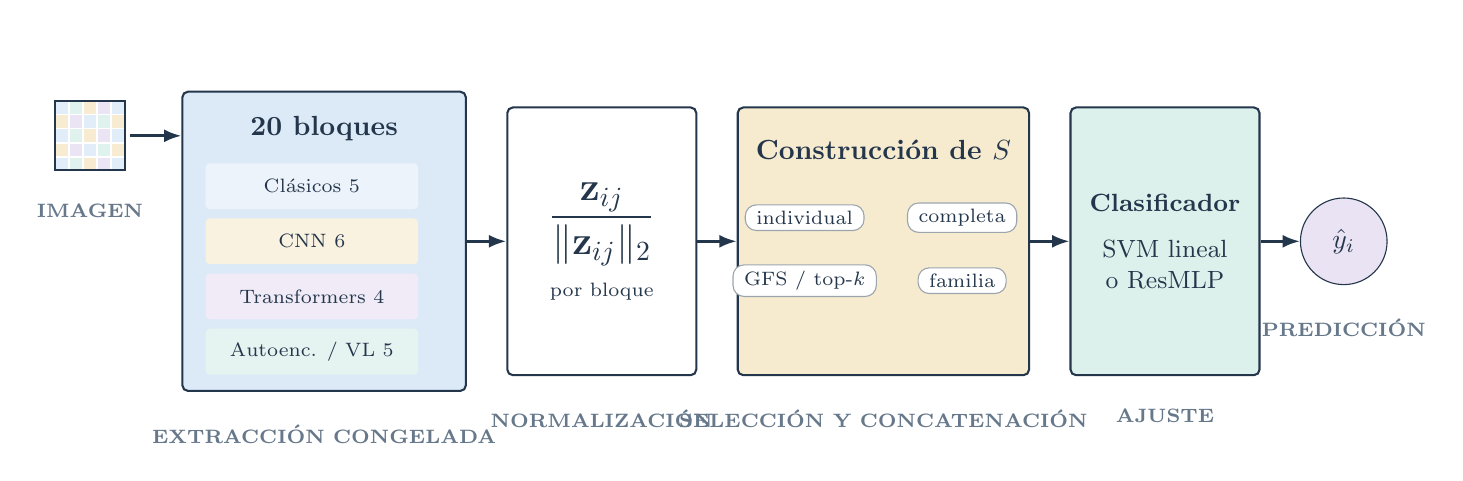
\begin{tikzpicture}[font=\small,node distance=5mm]
  % Input texture: a restrained symbolic swatch.
  \foreach \r in {0,...,4}{\foreach \c in {0,...,4}{
    \pgfmathtruncatemacro{\k}{mod(2*\r+\c,4)}
    \ifcase\k\def\cc{blue!85}\or\def\cc{teal!90}\or\def\cc{amber!95}\or\def\cc{violet!95}\fi
    \fill[\cc] (0.18*\c,0.18*\r) rectangle ++(0.16,0.16);
  }}
  \draw[ink,line width=.7pt] (0,0) rectangle (.88,.88);
  \node[phase,below=3mm] at (.44,0) {IMAGEN};

  \node[stage,fill=blue,minimum width=36mm,minimum height=38mm,anchor=west] (bank) at (1.6,-.9) {};
  \node[font=\bfseries,text=ink,anchor=north] at ([yshift=-2mm]bank.north) {20 bloques};
  \node[family,fill=blue!55,anchor=west] at ([xshift=3mm,yshift=7mm]bank.west) {Clásicos \hfill 5};
  \node[family,fill=amber!65,anchor=west] at ([xshift=3mm,yshift=0mm]bank.west) {CNN \hfill 6};
  \node[family,fill=violet!70,anchor=west] at ([xshift=3mm,yshift=-7mm]bank.west) {Transformers \hfill 4};
  \node[family,fill=teal!75,anchor=west] at ([xshift=3mm,yshift=-14mm]bank.west) {Autoenc. / VL \hfill 5};
  \node[phase,below=3mm of bank] {EXTRACCIÓN CONGELADA};

  \node[stage,fill=white,minimum width=24mm,right=of bank] (norm)
    {\Large $\displaystyle\frac{\mathbf z_{ij}}{\lVert\mathbf z_{ij}\rVert_2}$\\[1.8mm]\scriptsize por bloque};
  \node[phase,below=3mm of norm] {NORMALIZACIÓN};

  \node[stage,fill=amber,minimum width=37mm,right=of norm] (compose) {};
  \node[font=\bfseries,text=ink,anchor=north] at ([yshift=-3mm]compose.north) {Construcción de $S$};
  \node[tag,anchor=center] at ([xshift=-10mm,yshift=3mm]compose.center) {individual};
  \node[tag,anchor=center] at ([xshift=10mm,yshift=3mm]compose.center) {completa};
  \node[tag,anchor=center] at ([xshift=-10mm,yshift=-5mm]compose.center) {GFS / top-$k$};
  \node[tag,anchor=center] at ([xshift=10mm,yshift=-5mm]compose.center) {familia};
  \node[phase,below=3mm of compose] {SELECCIÓN Y CONCATENACIÓN};

  \node[stage,fill=teal,minimum width=24mm,right=of compose] (clf)
    {\bfseries Clasificador\\[2mm]SVM lineal\\o ResMLP};
  \node[phase,below=3mm of clf] {AJUSTE};

  \node[draw=ink,circle,fill=violet,minimum size=11mm,right=5mm of clf,font=\bfseries,text=ink] (pred) {$\hat y_i$};
  \node[phase,below=3mm of pred] {PREDICCIÓN};

  \draw[flow] (.95,.44) -- (bank.west |- 0,.44);
  \draw[flow] (bank.east) -- (norm.west);
  \draw[flow] (norm.east) -- (compose.west);
  \draw[flow] (compose.east) -- (clf.west);
  \draw[flow] (clf.east) -- (pred.west);
  % Protected whitespace required by the research-mode visual QA title band.
  \path ([yshift=8mm]current bounding box.north) coordinate (topPadding);
\end{tikzpicture}
\end{document}
